\documentclass[handout,10pt]{beamer}
\usepackage{SexySlides1,fancyvrb,outlines,pbox}

\definecolor{UniBlue}{RGB}{83,121,170}
\setbeamercolor{title}{fg=UniBlue}
\setbeamercolor{frametitle}{fg=UniBlue}
\newcommand{\colubf}{\color{UniBlue} \bf}

%% smart verbatim
\fvset{framesep=1cm,fontfamily=courier,fontsize=\scriptsize,framerule=.3mm,numbersep=1mm,commandchars=\\\{\}}

\title[Envelopes in Chemometrics]
{\Large  
Modeling Mutagenicity Status\\of a Diverse Set of Chemical Compounds\\by Envelope Methods
}

\author[]
{Subho Majumdar}

\institute[]
{School of Statistics, University of Minnesota} 

\date [December 12, 2013]

%%%%%%%List Outline in the beginning of each section.
\AtBeginSection[] {
   \begin{frame}
       \frametitle{Outline}
       \tableofcontents[currentsection]
   \end{frame}
}

%-------------------------------------------------------------------
\begin{document}

%\begin{frame}
\frame{ \titlepage}
%\end{frame}

\frame{\frametitle{Table of contents}\tableofcontents}

%---------------------------------------------------
\section{The data and the variables}

\begin{frame}
\frametitle{The data}
\begin{itemize}
\item The data were taken from the CRC Handbook of Identified Carcinogens and Non-carcinogens.

\item The response variable is 0/1 mutagen status obtained from \textit{Ames test of mutagenicity}. A chemical compound was classified as mutagen (scored 1) if its Ames score exceeded a certain cutoff, non-mutagen (scored 0) otherwise.

\item Total 508 compounds- 256 mutagens and 252 non-mutagens.

\item The dataset is diverse, meaning that chemical compounds belong to different chemical classes, some fairly different from each other, like Alkanes and Amines.
\end{itemize}
\end{frame}

\begin{frame}
\begin{figure}\begin{center}
   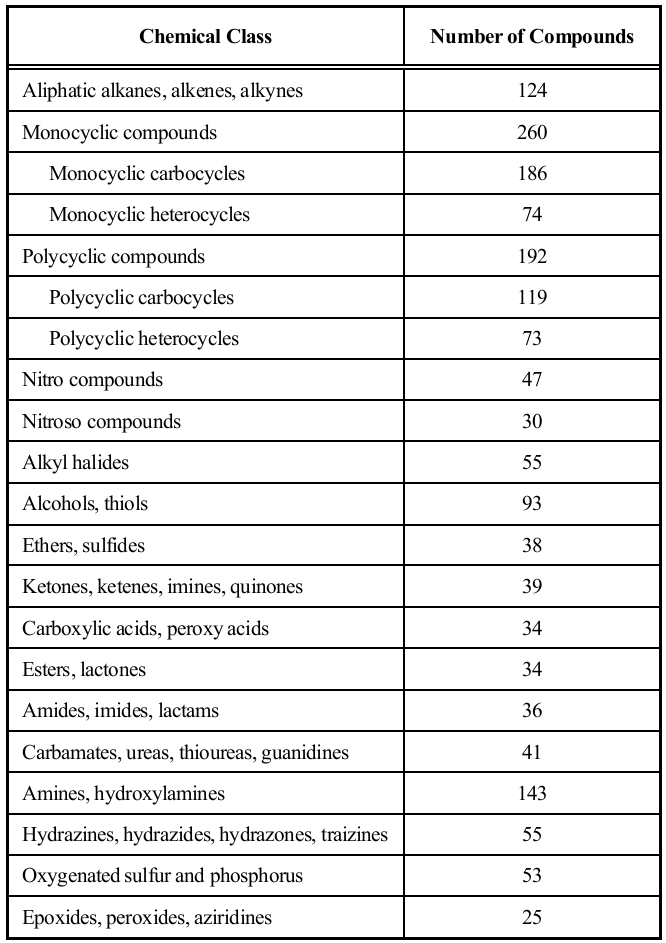
\includegraphics[height=8cm]{class.png}
   \label{fig:fig1}
\end{center}\end{figure}
\end{frame}

\begin{frame}
\frametitle{Description of variables}
Four types of variables:\vspace{.5cm}
\begin{enumerate}
\item \textbf{Topostructural (TS)}- Define the molecular topology, i.e. connectedness of atoms within a molecule (103 descriptors).
\vspace{.2cm}
\item \textbf{Topochemical (TC)}- Have information on atom and bond types (195 descriptors).
\vspace{.2cm}
\item \textbf{3-dimensional (3D)}- Define 3-dimensional aspects of the overall molecular structure (3 descriptors).
\vspace{.2cm}
\item \textbf{Quantum-Chemical (QC)}- Electronic aspects of molecular structure (6 descriptors).
\end{enumerate}
\end{frame}

\begin{frame}
\frametitle{Previous work}
\begin{itemize}
\item Use of {\colbbf Ridge Regression} to build a predictive model of mutagenicity (\textit{Hawkins et al, 2004}). The 0/1 mutagenicity score was used as response variable since 1 corresponds to a higher mutagenicity score and 0 corresponds to a lower one.
\vspace{0.5cm}
\item {\colbbf Variable selection} on a larger set of predictors by adapting a supervised clustering algorithm previously used on high-dimensional genetic data (\textit{Majumdar et al, 2013}).
\end{itemize}
\end{frame}

\section{Fitting Envelope models}

\begin{frame}
\frametitle{The Envelope regression model (\textit{Cook, Li and Chiaromonte, 2010})}
$$ \bfY_i = \bfalpha + \bfbeta\bfX_i + \bfepsilon_i,\quad \bfepsilon_i\sim N(\bfZero,\bfSigma) \mbox{ with }\bfSigma = \bfGamma\bfOmega\bfGamma^T + \bfGamma_0\bfOmega_0\bfGamma^T$$
$$ i = 1,2,...,n $$
\begin{itemize}
\item $\bfY\in\BR^{r\times n}$ multivariate response vector, $\bfX\in\BR^{p\times n}$ \textit{non-stochastic predictors}.
\item $\bfalpha\in\BR^r$ intercept, $\bfbeta\in\BR^{r\times p}$ matrix of regression coefficients: both unknown.
\item $\bfGamma\in\BR^{r\times u},\bfGamma_0\in\BR^{r\times (r-u)}$ semi-orthogonal basis matrices of $\cE_\bfSigma(\cB)$ and its orthogonal complement, respectively, with $\cB = \mbox{span}(\bfbeta)$ and $0\leq u\leq r$ being the dimension of the envelope.
\item $\bfOmega = \bfGamma\bfSigma\bfGamma^T, \Omega_0 = \bfGamma_0\bfSigma\bfGamma_0^T$ coordinate matrices corresponding to $\bfGamma, \bfGamma_0$.
\end{itemize}
\end{frame}

\begin{frame}
\frametitle{Enveloping the predictors}
\begin{itemize}
\item \textit{Stochastic predictors}, distributed as i.i.d. $N(\bfmu_\bfX,\bfSigma_\bfX)$.
\vspace{.2cm}
\item $\bfSigma_\bfX = \bfPhi\bfOmega\bfPhi^T + \bfPhi_0\bfOmega_0\bfPhi_0^T$, with $\bfPhi\in\BR^{p\times q}, \bfPhi_0\in\BR^{p\times(p-q)}, 0\leq q\leq p$ being semi-orthogonal basis matrices of the envelope of span($\bfbeta^T$) and its orthogonal complement, respectively.
\vspace{.2cm}
\item $\bfOmega = \bfPhi\bfSigma_\bfX\bfPhi^T, \Omega_0 = \bfPhi_0\bfSigma_\bfX\bfPhi_0^T$ coordinate matrices corresponding to $\bfPhi, \bfPhi_0$.
\end{itemize}
\end{frame}

\begin{frame}
\frametitle{Envelope regression model for our data: basics}
\begin{itemize}
\item log-transformed data.
\vspace{.2cm}
\item the predictors taken as multivariate response, and the 0/1 mutagenicity status taken as the single predictor, and then envelope regression models are obtained.
\vspace{.2cm}
\item Hierarchical approach to observe the effect of adding different classes of predictors: separate envelope models fit on data with only TS, only TC, TC + TS and full set of predictors.
\end{itemize}
\end{frame}

\begin{frame}
\frametitle{Envelope regression model for our data: rank-deficiency}
\begin{itemize}
\item Even after log-transformation the data remains rank-deficient in nature, so envelope models cannot be fit on the actual data.
\vspace{.2cm}
\item For each set of variables, at first Principal Component Analysis is done on the data-matrix, and then envelopes are fit on the minimum number of principal components that explain $\geq 90\%$ of the total variation.
\vspace{.2cm}
\item The coefficient estimates for original variables and their asymptotic standard errors are then obtained from their envelope counterparts by back-transformation.
\end{itemize}
\end{frame}

\begin{frame}
\frametitle{Getting back coefficient estimates and standard errors}
Suppose $\bfY\in\BR^{r\times n}$ is the original matrix of multivariate responses, and $\bfL\in\BR^{r\times k}$ is the PC loading matrix. Thus the transformed predictors are $\bfL^T\bfY$. $\bfb\in\BR^{k \times 1}$ is the envelope estimator of coefficients of PCs in our case, so that for $i=1,...,k$
$$ b_i \sim N(\bfl^T_i\beta,\nu^2_i) $$
with $\nu^2_i$ being the $i$-th diagonal element of $\bfL\bfSigma\bfL^T$, and $\bfl_i$ the $i$-th column of $\bfL$.\\
\vspace{.5cm}
Thus the vector $\bfL\bfb$ gives the estimate of coefficients of original variables, and $\sum_{i=1}^k l_{ji}^2\hat\nu_i^2$ estimates the variance of its $j$-th coordinate, $j = 1,...,r$.
\end{frame}

\begin{frame}
\frametitle{Results: Variance reduction by envelopes}
In all the envelope models, there were massive gains in terms of variation. The gains were especially large for the first 2 principal components.
\vspace{.2cm}

\begin{scriptsize}
\begin{table}\centering
    \begin{tabular}{|c|c|c||c|c|c|c|c|c|}\hline
    \textbf{Set of} & \textbf{No. of} & \textbf{Envelope} & 
    \multicolumn{3}{c|}{\textbf{\% variance explained by}} & \multicolumn{3}{c|}{\textbf{Envelope gain ratios for}}\\\cline{4-9}
    \textbf{descriptors}                  & \textbf{PCs}                                                 & \textbf{dimension} ($u$) & \textbf{PC1}                      & \textbf{PC2}   & \textbf{PC3}  & \textbf{PC1}                & \textbf{PC2}   & \textbf{PC3}  \\\hline\hline
    \textbf{TS}                 & 7                                                 & 3                        & 70.43                    & 10.35 & 2.60 & 25.91              & 36.17 & 2.10 \\ \hline
    \textbf{TC}                 & 8                                                 & 4                        & 75.89                    & 6.52  & 2.42 & 15.40              & 35.26 & 1.00 \\\hline
    \textbf{TS + TC}            & 13                                                & 6                        & 70.27                    & 7.94  & 2.21 & 10.40              & 37.99 & 1.22 \\\hline
    \textbf{Full} & 15 & 11 & 58.19 & 7.60 & 5.98 & 1.00 & 1.00 & 1.00 \\\hline
    \end{tabular}
\end{table}
\end{scriptsize}
\vspace{.2cm}
\textbf{Note}:
\begin{itemize}
\item With default tolerances of objective and gradient function in \texttt{env} the algorithm did not converge in 1000 iterations. For this reason they were set to \texttt{1e-7} and \texttt{1e-4}.
\vspace{.2cm}
\item As far as other PCs of full model were concerned, PCs 9, 11, 13 and 15 gave 1.26, 1.96, 1.88 and 1.5-fold gains, respectively.
\end{itemize}
\end{frame}

\begin{frame}
\frametitle{Results: significant predictors}
\begin{scriptsize}
\begin{table}\centering
    \begin{tabular}{|c|c|c|c|}\hline
    Set of      & \multicolumn{2}{c|}{No. of descriptors} & Significant\\\cline{2-3}
    descriptors & Total              & Significant & PCs\\\hline\hline
    TS          & 103                & 51         & 4, 5, 7 \\\hline
    TC          & 195                & 98         & 1, 3, 8\\\hline
    TS + TC     & 298                & 89         & 4, 7, 11\\\hline
    Full        & 307                & 56         &  2, 3, 8, 10, 14\\\hline
    \end{tabular}
\end{table}
\end{scriptsize}

\begin{itemize}
\item For envelope models on only TS or only TC data, correlated predictors have a tendency to all have significant $t$-ratios.
\item When the two types of variables are combined, there is less linear dependency among significant predictors.
\end{itemize}
\end{frame}
\section{Performance of envelopes in prediction}

\begin{frame}
\frametitle{Procedure: Envelope Linear Discriminant Analysis}
\begin{enumerate}
\item Use the envelope basis matrix $\hat\bfGamma$ to reduce the predictors.
\vspace{.2cm}
\item Then use the transformed predictors $\hat\bfGamma^T\bfL^T\bfY$ to do Linear Discriminant Analysis, and use that rule to predict class of new samples.
\vspace{.2cm}
\item Correct classification percentages are obtained through cross-validation on the full sample.
\vspace{.2cm}
\item Leave-one-out CV in place of $k$-fold as predictions can vary across different samples of folds because of diverse nature of the dataset.
\end{enumerate}
\end{frame}

\begin{frame}
\frametitle{Method of Cross-validation}
\begin{center}\begin{large}
{\colubf Na\"{i}ve CV vs. Two-fold CV}
\end{large}\end{center}
\begin{figure}\begin{center}
   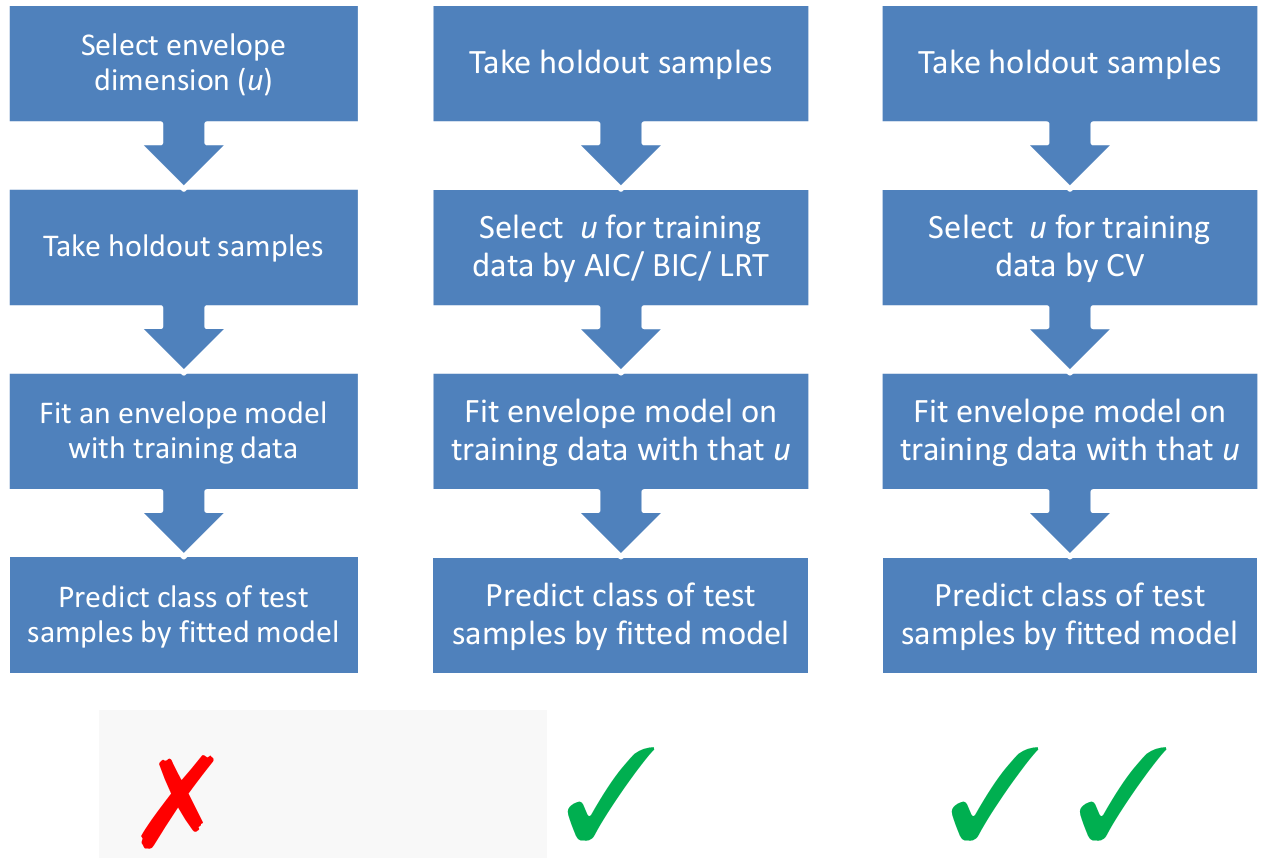
\includegraphics[height=7cm]{cv.png}
   \label{fig:fig1}
\end{center}\end{figure}
\end{frame}

\begin{frame}
\frametitle{Performance of envelopes in prediction}
\begin{scriptsize}
\begin{table}\centering
    \begin{tabular}{|c|c|c|c|c|c|}
    \hline
    \textbf{Model}                                     & \textbf{Type of predictors} & \textbf{No. of}     & \multicolumn{3}{c|}{\textbf{Correct classification} \%}\\\cline{4-6}
    \textbf{description}                               & \textbf{in model}           & \textbf{predictors} & \textbf{Total}                     & \textbf{Mutagens} & \textbf{Non-mutagens} \\ \hline
    Ridge regression                          & TS+TC              & 298        & 76.97                     & 83.98    & 69.84        \\ \hline
    Ridge regression                          & TS+TC+3D+QC        & 307        & 77.17                     & 84.38    & 69.84        \\ \hline
    \pbox{10cm}{Ridge regression after \\variable selection} & TS+TC+AP           & 203        & 78.35                     & 84.38    & 72.22        \\ \hline\hline
                                  & TS                 & 103        & 57.09                     & 65.63    & 48.41        \\\cline{2-6}
    Envelope LDA                                         & TC                 & 195        & 58.27                     & 69.92    & 46.43        \\\cline{2-6}
    ~                                         & TS+TC              & 298          & 60.24 & 69.14        & 51.19            \\ \hline
    \end{tabular}
\end{table}
\end{scriptsize}
\end{frame}

\section{Conclusion}

\begin{frame}
\frametitle{Discussion}
\begin{outline}
\1 For estimation, envelope models performed really well in conjunction with PCA for rank-deficient data, offering heavy gains for the major principal components over OLS.
\vspace{.2cm}
\1 Possible reason for the poor performance in prediction:
\2 High material to immaterial variation ratio
\2 Heteroskedasticity caused by diverse chemical classes among compounds
\2 Variation of scales between different types of variables
\vspace{.2cm}
\1 {\colubf 3D plot of PCs in MATLAB}
\vspace{.2cm}
\1 A more detailed formulation should improve the predictive performance of envelope models.
\vspace{.2cm}
\1 Logistic Envelope Regression.
\end{outline}
\end{frame}

\begin{frame}
\frametitle{Acknowledgements}
\begin{itemize}
\item Prof. Dennis Cook, for his guidance and valuable inputs.
\vspace{.2cm}
\item Henry Zhang, for providing his codes for logistic envelope regression.
\vspace{.2cm}
\item Greg Grunwald, UofM-Duluth for providing the dataset.
\end{itemize}
\end{frame}

\begin{frame}
\frametitle{References}
\hspace{.2cm}Cook, R.D.; Li B.; Chiaromonte F. Envelope models for parsimonious and efficient Multivariate Linear Regression. \textit{Stat. Sinica}, \textbf{2010}, 20, 927-1010.\\
\vspace{.2cm}
\hspace{.2cm}Hawkins, D.M.; Basak, S.C.; Mills, D. QSARs for chemical mutagens from structure: ridge regression fitting and diagnostics. \textit{Environ. Toxicol. Pharmacol.}, \textbf{2004}, 16, 37-44.\\
\vspace{.2cm}
\hspace{.2cm}Majumdar S.; Basak S.C.; Grunwald G.D. Adapting Interrelated Two-Way Clustering Method for Quantitative 
Structure-Activity Relationship (QSAR) Modeling of Mutagenicity/ Non-Mutagenicity of a Diverse Set of Chemicals. \textit{Curr. Comput. Aided Drug Des.}, \textbf{2013}, 9, 000-000.

\end{frame}
%\begin{frame}
%\frametitle{Description of variables}
%The first 5 questions are concerned with drinking and driving, the next 5 with other drug use, and the last two with sexual behavior. Also, QN29, QN40, QN44 and QN57 have a time component.
%
%\begin{figure}\begin{center}
%   \includegraphics[height=6cm]{hw231.png}
%   \label{fig:fig1}
%\end{center}\end{figure}
%\vspace{.5cm}
%\end{frame}

%\begin{frame}[fragile]
%\frametitle{Proportion of positive responses for each question}
%For the sake of simplicity only those cases that were fully observed are used in the analysis. Using those cases, the proportion of respondents who answered yes to each of the 12 questions are found as below:
%\begin{block}{}
%\begin{Verbatim}
%> load(url("http://tinyurl.com/yrbs05-rda"))
%> len = dim(yrbs05)[1]
%> probs = 1-(apply(yrbs05[,1:12], 2, sum) - len)/len; probs
%\textbf{      QN29       QN34       QN11       QN40       QN42       QN45       QN48 }
%\textbf{0.15757455 0.12945048 0.11319438 0.25132143 0.28473123 0.08935873 0.08935873 }
%\textbf{      QN50       QN52       QN53       QN58       QN59 }
%\textbf{0.11917822 0.06053655 0.05953924 0.06891393 0.16814601 }
%\end{Verbatim}
%\end{block}
%\end{frame}

%\begin{frame}[fragile]
%\frametitle{Fitting a model of complete independence}
%Following are the estimated probabilities for all 12 questions. Note that they are same as the probabilities in the last section.
%\begin{columns}[c]
%\column{1.5in}
%\begin{block}{}
%\begin{Verbatim}
%$QN29
%           Pr(1)  Pr(2)
%class 1:  0.1576 0.8424
%
%$QN34
%           Pr(1)  Pr(2)
%class 1:  0.1295 0.8705
%
%$QN11
%           Pr(1)  Pr(2)
%class 1:  0.1132 0.8868
%
%$QN40
%           Pr(1)  Pr(2)
%class 1:  0.2513 0.7487
%
%$QN42
%           Pr(1)  Pr(2)
%class 1:  0.2847 0.7153
%
%$QN45
%           Pr(1)  Pr(2)
%class 1:  0.0894 0.9106
%
%\end{Verbatim}
%\end{block}
%
%\column{1.5in}
%\begin{block}{}
%\begin{Verbatim}
%$QN48
%           Pr(1)  Pr(2)
%class 1:  0.0894 0.9106
%
%$QN50
%           Pr(1)  Pr(2)
%class 1:  0.1192 0.8808
%
%$QN52
%           Pr(1)  Pr(2)
%class 1:  0.0605 0.9395
%
%$QN53
%           Pr(1)  Pr(2)
%class 1:  0.0595 0.9405
%
%$QN58
%           Pr(1)  Pr(2)
%class 1:  0.0689 0.9311
%
%$QN59
%           Pr(1)  Pr(2)
%class 1:  0.1681 0.8319
%\end{Verbatim}
%\end{block}
%\end{columns}
%\end{frame}

\begin{frame}
\centering\huge
\textcolor{UniBlue}{\textbf{THANK YOU!}}
\end{frame}

\end{document} 

